\chapter{CFR-D and Decomposition}
\label{ch:cfr-d}
\note{
  This chapter summarizes the approach, methods and results of~the authors~\cite{BurchJohansonBowling13}.
}

\section{Motivation}
The work of~(\cite{BurchJohansonBowling13}) describes a~pioneering technique how to \emph{decompose} subgames of~imperfect-information games and solve them independently, while preserving the optimality of~the full-game solution.
Many benefits of~subgame re-solving are inherited from perfect-information games:
\begin{itemize}
  \item Run-time information (e.g. endgame actually reached during a~real play) can be exploited in a~smarter way.
  \item Memory and disk limitations (either at~run-time or while solving a~game) can be overcome by a~time/space trade-off.
  \item A~\acrlong{ne} for a~game larger than available storage may be computed.
  \item If we only need to work with one subgame at a~time, then significantly less storage is required.
  \item It is not obligatory to store the complete strategy, which might be too large to store.
    Instead, subgame strategies may be re-computed on~demand, when needed.
\end{itemize}

As for re-solving subgames in~the imperfect-information setting, all previous algorithms were limited to rather small domains, with the complete strategy that can fit in~available space.
As a~consequence, several appealing games still resist to be solved, despite the intensive effort put in~their research.
\note{
  This used to be the case for the two-player \acrshort{lhe}, until the~recent, highly-celebrated breakthrough by~the same research group (\cite{Bowling2015heads}).
}

\section{Gadget Game}
\epigraphLong{
  Dreams about the future are always filled with gadgets.
}{Neil deGrasse Tyson}
Again, we start by~creating a~fine-grained abstraction for the subgame.
The original strategy for the subgame (from the coarse abstraction) is then translated into the fine-grained abstraction as $\sigma_1^S$.
The translated strategy is now used to compute $CBV_2 ^{\sigma_1^S} (I)$ for every information set~$I$ at~the root of~the subgame.
These values will be useful for the gadget construction to~guarantee the safety of~the resulting strategy.
See Figure~\ref{fig:re-solving-gadget} for a~sketch of~the construction.

\begin{figure}[H]
  \centering
  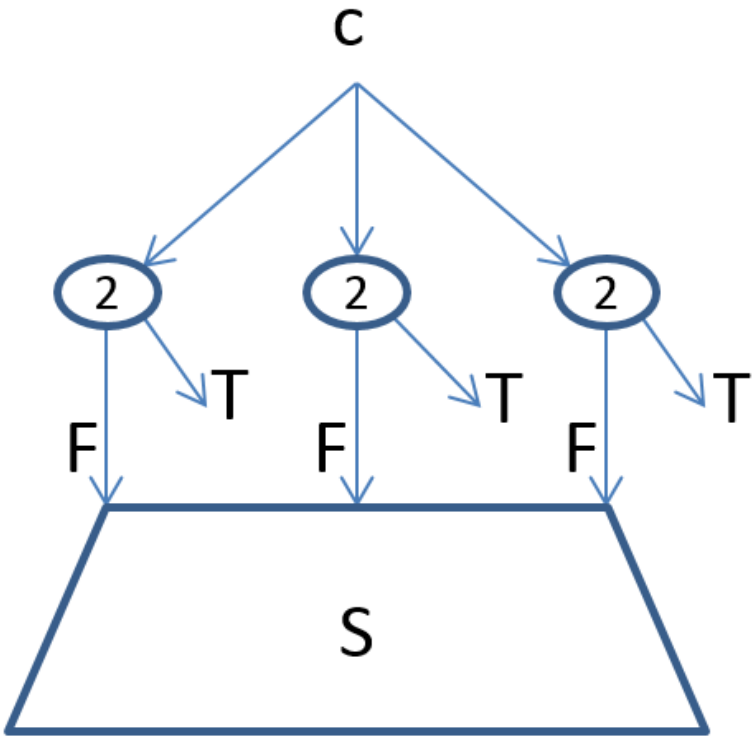
\includegraphics[width=.3\textwidth]{../img/re-solving-game-gadget.png}
  \def\captionTitle{A~gadget game for re-solving subgames}
  \caption[\captionTitle]{
    \captionTitle.
    The opponent chooses in~every state prior to the endgame either to (F)ollow the action into the endgame, or to (T)erminate.
    His utility after the (T)erminal action is set to his counterfactual best response in that state.
  }
  \label{fig:re-solving-gadget}
\end{figure}

To construct the gadget, we add one chance node at~the root of~the game, followed by additional nodes for player~$2$:
one for every state at~the root of the subgame.
At~each of~these nodes, $2$ may either accept the corresponding counterfactual best response value calculated earlier, or play the subgame (to get to the corresponding state at~the root of~the subgame).
The chance player distributes the player~$2$ into these states using the (normalized) $\pi^\sigma_{-2}$ (how likely is the state given that $2$ plays to reach it).
Since the game is zero-sum, this forces player~$1$ to play the subgame well enough, so that the opponent's value is no greater than the original CBV.
For more details see (\cite{BurchJohansonBowling13}).

\section{Equivalent Linear Program}
\begin{equation}
  \label{lp:cfr-d}
  \begin{split}
    \max_{v, x}\ &0 \\
    \color{red}
      v_I - m &
    \color{red}
      \ge CBV_2^\sigma(I), \quad I \in \I_2^{R(S)}\\ 
    Ex &= e \\
    F^\top v - A^\top x &\le \vect{0} \\
    x &\ge \vect{0},
  \end{split}
\end{equation}

\section{Discussion}
The innovative aspect of~(\cite{BurchJohansonBowling13}) consists of~two main contributions:
\begin{itemize}[(i)]
  \item A~technique to re-solve imperfect-information subgames, which is guaranteed not to increase sub-optimality of~the resulting full-game strategy.
    Owing to summary information about a~subgame strategy (namely the \acrlong{cbv}s), the newly generated strategy is no more exploitable than the original one.

  \item A~new off-line solving algorithm called \emph{\acrfull{cfr-d}}, capable of~computing an~error-bounded \acrshort{ne} approximation.
    \acrshort{cfr-d} achieves this by decomposing and independently analyzing subgames.

    By~sacrificing computation time, the decomposition allows for \emph{sub-linear space costs}.
    For instance, two-player \acrshort{lhe} with \acrshort{cfr-d} can be solved in less than 16 GB, rather than~more than 200 TB of~disk space!
\end{itemize}
